\documentclass[10pt,a4paper]{article}
\usepackage[UKenglish]{babel}
\usepackage[latin1]{inputenc}
\usepackage{geometry}
\usepackage{amsmath}
\usepackage{amsfonts}
\usepackage{amssymb, mathabx}
\usepackage{graphicx}
\usepackage{appendix}
\usepackage[usenames,svgnames, table]{xcolor}
\usepackage{fancyvrb}
\usepackage{tabularx}
\usepackage{tcolorbox}
\tcbuselibrary{skins,breakable}
\usetikzlibrary{shadings,shadows}
\usepackage[ampersand]{easylist}
\usepackage[breaklinks]{hyperref}
\hypersetup{%
	colorlinks=true,
	citecolor=DarkGreen,
	linkcolor=DarkBlue,
	urlcolor=DarkRed,
	pdfborder= 0 0 0
}


\geometry{verbose,tmargin=1in,bmargin=1in,lmargin=1in,rmargin=1in}

\title{A guide to oskar}
%\subtitle{for running and recording experiments with LabVIEW and HDF5}
\author{a.deller@ucl.ac.uk}
\date{\today}

\definecolor{light-gray}{gray}{0.9}
\definecolor{lighter-gray}{gray}{0.98}

\newenvironment{warning}[1]{%
	\tcolorbox[beamer,%
	breakable,
	colback=white,colframe=DarkRed,%
	title=Warning:]}%
{\endtcolorbox}

\begin{document}
\maketitle
\tableofcontents

\section{Introduction, Acknowledgements, and Excuses.}
oskar \footnote{Tenuous acronym: Orchestrate Sequences. Keep Attribute Record} is a collection of tools written using LabVIEW 2013 \footnote{LabVIEW is a registered trademark of \href{http://www.ni.com/}{National Instruments}.}. It is designed to assist in coordinating hardware control and to provide a framework for acquired data using \href{https://www.hdfgroup.org/why_hdf/}{HDF5} Hierarchical Data Format (HDF)\footnote{HDF is a trademark of the \href{http://www.hdfgroup.org/}{HDF group}.}.  Essentially, it is a tool for running experiments. It was designed with a focus on: extensibility (it should be reasonably easy to add new control/ DAQ hardware); on sensibly structuring acquired data; and explicitly pairing data with the metadata (attributes) needed to describe it.

The code was written by Adam Deller at University College London for experiments in laser spectroscopy of positronium. Some features are conceptually based on a program he developed at Swansea University (openseq), which was originally inspired by a similar system invented by Aled Isaac.  Many of the features of openseq were hashed out with feedback and help from Tim Mortensen. Much of the testing of oskar was done by Ben Cooper and Alberto Munoz Alonso.    HDF5 support is provided by the \href{http://h5labview.sourceforge.net/}{h5labview} library developed by Martijn Jasperse.

To make use of oskar some experience writing in G (Labview code) is essential. The project is useless without control hardware and data acquisition devices, however, no drivers have been included. You will need to interface any drivers (e.g., using  LINX by \href{https://www.labviewmakerhub.com}{LabVIEW MakerHub} to control an  \href{https://www.arduino.cc/}{Arduino}) with oskar yourself -- fortunately, this is a fairly simple process and examples are included.  In the data acquisition examples crudely simulated oscilloscopes and cameras are used.  Once you have successfully  interfaced the drivers you need, sequencer.vi solves the problem of covering large parameter spaces systematically and flexibly.  There is very little going on under the hood (see section~\ref{sex:seq} for an overview, or appendix~\ref{sex:pseudo} for a simplistic pseudo-code version),  nonetheless you will need a decent grasp of LabVIEW to be able to inspect the code and modify it to suit your needs.

Also, please bear-in-mind that I am not a professional LabVIEW developer and none of the VIs are necessarily examples of good coding practice. Though I've found oskar is generally very stable and easy to use (once you know the basics), be sure to test everything thoroughly for yourself and be vigilant for unexpected behaviour!
\section{Installation}
oskar requires LabVIEW 2013 (or higher) Full Development Edition (written using 32-bit version
on Windows 7 64-bit). The DAQ example fake\_camera.vi needs the \href{http://www.ni.com/downloads/}{NI Vision Development Module}.

\begin{itemize}

\item  Install \href{https://www.hdfgroup.org/HDF5/release/obtain5.html}{HDF5}. Select 32-bit/ 64-bit version to match LabVIEW install. Reboot.

\item Download the latest version of the \href{https://sourceforge.net/projects/h5labview/files/}{h5labview library} and install it using the using  \href{http://vipm.jki.net/}{JKI VI package manager}. 

\item Download and unzip \href{https://github.com/PositroniumSpectroscopy/oskar}{oskar}. Open oskar.lvproj.

\end{itemize}

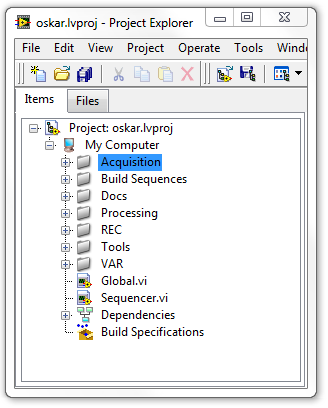
\includegraphics[width=0.3\textwidth]{images/oskar.png}

\emph{Recommended:}
\begin{itemize}
	\item NI VISA (hardware drivers)
	\item  \href{https://www.hdfgroup.org/products/java/hdfview/}{HDFView} (for opening and exploring HDF5 files).
\end{itemize}

There are many freely available libraries for importing hdf5 data for analysis, e.g., \href{http://www.h5py.org/}{h5py} for python.

\section{The Sequencer and VARs}
\subsection[Sequencer.vi]{\label{sex:seq}Sequencer.vi \\ %
	\normalsize - a tool for conducting experimental series}

\subsubsection{History}
The openseq version of sequencer.vi was written to parse configuration files for digital output from an FPGA and tables for an analogue output device, which together were used to control a series of electrodes for a positron trap\footnote{J. Clarke \emph{et al.} (2006), \emph{Rev. Sci. Instrum.} \textbf{77}, 063302.}.  The program acted as a bridge between the simple text files and device drivers, providing a way to automatically run series of experiments where timings and voltages could be systematically varied. Later, a simple system for control of ancillary devices (e.g. a waveform generator) was integrated into the sequencer using VARS.  This VARS system was designed to flexibly accommodate any number of additional devices without requiring modification to the sequencer.vi code  (see below), and extended its power to control of devices across a network.  The sequencer.vi is most powerful when used in combination with modder.vi.  The latter was written to automatically generate thousands of sequences for investigating \emph{very} large parameter spaces. 

As well as conducting control of hardware, the sequencer is used as a hub for a data acquisition framework based on the HDF5 format.  By generating unique run IDs (RID) and hdf5 files for every series of experiments it executes, the sequencer can coordinate programs written for data acquisition (e.g. from cameras/ oscilloscopes) and organise the recording of data files into a structure suitable for batch analysis.

This simplified version of sequencer.vi included in oskar has been written for generically conducting experiments/ data acquisition with control over many variables.   No hardware drivers are included, however, the VARs and data acquisition system can be rapidly adapted to control/ coordinate fairly complex experiments.

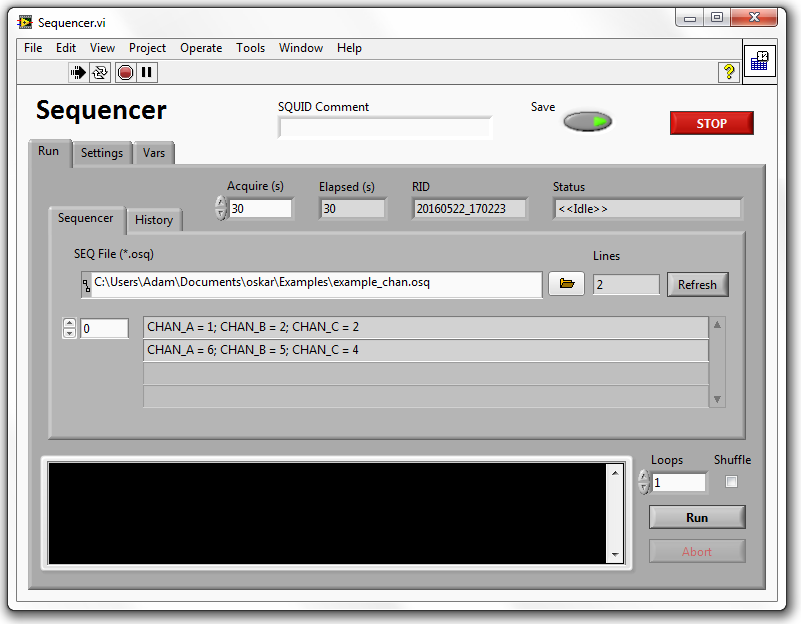
\includegraphics[width=0.75\textwidth]{images/sequencer.png}

\subsubsection{Overview}

The basic premise of sequencer.vi is to read experimental scripts, i.e., sequence files (see below), which describe how parameters should be changed during a measurement series.  The program then ensures that the requested conditions (VARS) are met at the right time, and that any data acquisition software is informed of how to save data so that it can be mapped back to these conditions.  sequencer.vi is effectively the \emph{conductor} of an experimental measurement and does not perform the actual hardware communication (which is delegated to individual VAR vi's). This modulat approach makes extending control to new instruments relatively painless.

\subsubsection{Sequence files}
The sequence file (*.osq) provides a means to script a simple experiment. Every \emph{line} contains a single configuration of the experimental variables that one wishes to set, and recorded data is mapped to these using a sequence ID (SQUID) that iterates as each configuration is executed in turn.

The osq files are stored as xml and each \emph{line} is an element of an array called \emph{SEQs}.  Each of these elements are clusters that, in the simplest case (see section~\ref{sex:ext} for possible extensions), contain only a string called \emph{Comment} and an array called \emph{VAR Array}. The former does nothing but provide a way to add a comment to each line; the latter is a two column string array: the first column contains every VAR name relevant to a given experiment and the second each corresponding value.  This cluster is called  a sequence \emph{line}, each of which correspond to one measurement configuration of variables.  A series of lines make up the sequence (i.e., a collection of measurement conditions), the execution of which constitutes an experimental RUN.  As a simple example, use Editor.vi to open and view the file \emph{./Examples/example\_seqs.osq}.  This sequence contains just two lines, each with a single VAR called PAUSE, with a value set to 1000 then 2000.

A sequence file is loaded into sequencer.vi by entering its file path into  \emph{SEQ File (*.osq)} on the \emph{Run/Sequencer} tab.  Loading a file will automatically count the number of \emph{lines} and will indicate the names and values of VARs in the series; this list is updated by pressing \emph{Refresh}.  The parameter \emph{Acquire} should be set to the amount of time that data will be recorded for per line before proceeding to the next. \emph{Loops} sets the number of times that the sequencer should loop over the whole series. 

When \emph{Run} is pressed (with an osq file successfully loaded) a time-stamp is used to create a RID (\%Y\%m\%d\_\%H\%M\%S) that uniquely identifies the measurement series. The sequencer then reads the XML file and proceeds by demanding that the desired experimental conditions of the first line (SQUID = 1) are met, after which it waits for the acquisition period to complete (i.e. \emph{Elapsed} $>$ \emph{Acquire}), then continues to the following line (SQUID = 2), and so forth until all lines have been run for all requested loops.  For details of how VARs are met, see section~\ref{sex:var}.  If \emph{shuffle} is selected when run is pressed then the lines are randomly reordered at the start of every loop, thus successive loops will be ordered differently.

The `History' Tab contains a list of all sequence file names and the times which they were run.  You can cycle \emph{SEQ File (*.osq)} over previously ran files by hovering over it and scrolling your mouse wheel (press `Refresh' to reload the sequence).

\subsubsection{Saving}
The folder `./[YYYY]/[MM]/[DD]/[RID]/', wherein a copy of the osq and the `[RID]\_raw.h5' file relating to a given run are recorded, is built during initialisation by date\_path\_h5.vi, using the RID and base(s) specified in the `Save Base' array (\emph{Settings} tab of sequencer.vi).   Specifying more than one base can be used to duplicate data recording.  This HDF5 file (or files) is that which data acquisition programs are directed to for recording data; the path is distributed by sequencer.vi using the global variable \emph{H5}.

When a run is started it will raise a dialogue that allows the user to record information regarding the ``Author" and ``Description".  This information is written to attributes of the data file.  Details written here often prove very useful during subsequent analysis. 

\subsection[VARs]{\label{sex:var}VARs \\ %
	\normalsize - controlling hardware with the sequencer}

\subsubsection{The principle}
The VARs system is used to control hardware with the sequencer.  To initialize every line of a sequence file, sequencer.vi becomes a VARs server -- effectively broadcasting the message: \emph{I don't care who you are or how you do it but I need each VAR from this list set to these values. Please let me know when it's done!}  More explicitly, for each line of a sequence the \emph{VAR Array}, e.g.

\hangindent=0.7cm
\rowcolors{1}{light-gray}{lighter-gray}
\emph{VAR array:} \\
\begin{tabularx}{0.3\textwidth}{X|X}
	\emph{Name} & \emph{Value} \\
	\hline
	VAR1 & value\_1 \\
	VAR2 & value\_2 \\
	\vdots & \\
	VAR$n$ & value\_$n$ \\
\end{tabularx}

\noindent is read and for each row of this array two Boolean columns are added: \emph{Received} and \emph{Set} (both initially set to False), as well as the string \emph{Options} (see below).  This new array is passed to a global variable and can be viewed on the tab \emph{Vars} in sequencer.vi.  For each row the sequencer waits for \emph{Received} to become True, then proceeds to the next row. After all VARs have been received the sequencer waits for all \emph{Set} values to be True (i.e. for every row of the array/ each requested VAR), before continuing to the acquisition stage.

Separate programs with control over the hardware corresponding to each VAR must be written which ``listen'' for requests from the sequencer.  The simple example of \emph{PAUSE} can be found in the VARs folder.  This vi listens for a VAR called PAUSE. Upon receiving the VAR from the sequencer it sets \emph{Received} in the global variable to true, then feeds the VAR value into a wait function (in ms). After waiting for the requested amount of time it updates \emph{Set} to true.  A similar example called \emph{HOLD} updates \emph{Set} when the user presses the button on its front panel (the VARs value is irrelevant). Use these examples as a template for making new VAR controls, replacing the code in the centre section with a subVI that can take the VAR value as an input, e.g. to set the current for a power supply/ wavelength of a  laser/ frequency of a waveform/ etc.  Use an output of the hardware control subVI to ensure the sequencer does not proceed until the desired hardware change has been completed. Note: any VAR hardware control programs should be added to the oskar project in order to have access to the global variables.

Options add flexibility to VAR control and can be used (optionally) by appending the VAR name with an underscore, e.g. VAR\_OPTION (for this reason, \emph{only} use underscores in VAR names for specifying options).  The sequencer splits the name at the underscore and transmits the name and option separately as individual strings.  It's up to the VAR vi to act on the option as appropriate.  For example, you could create a VAR control that can set the voltages on a channel of an AO device with VAR name `VOL'.  The option string could be interpreted as which channel to control. For this example

\hangindent=0.7cm
\rowcolors{1}{light-gray}{lighter-gray}
\emph{VAR array:} \\
\begin{tabularx}{0.3\textwidth}{X|X}
	\emph{Name} & \emph{Value} \\
	\hline
	VOL\_A & 5 \\
	VOL\_B & 10 \\
\end{tabularx}
\vspace{2mm}

\noindent the vi would first set channel A to 5 V then channel B to 10 V.  This is generally better than having separate VAR vi's for each channel as it forces the order they are set and prevents interference from simultaneous attempts to communicate with one device.  The options format can be used quite efficiently even with many channels, e.g., VAR\_1/2/3 could be used to build an array of AO voltages but only when a specific option is received (e.g., VAR\_update) will the commands be sent.  The level of sophistication in interpreting the options depends entirely on the VAR vi, and not on the sequencer. 

To see the VARs system in action try and run \emph{/Examples/example\_seqs.osq} with sequencer.vi -- be sure to have the VAR control \emph{PAUSE} running!  To see how options can be used with VARs try \emph{/Examples/example\_chan.osq} with \emph{CHANNEL.vi}. When testing VARs you may avoid saving by disabling the \emph{Save} option on the sequencer.vi front panel.

\subsubsection{The reality}

It's important to understand the technical details for how VARs are actually made in order to do something useful with them.  Open the template `PAUSE' and navigate to the block diagram.  There are 5 main sections to this code - namely:

\begin{enumerate}
	\item %
	Create a notifier based on the control `Var' (in this case: Var = ``PAUSE'').  This must match the notifier created by the Sequencer.
	\item %
	Wait for the notifier which, when received, will pass a value indicating the index of the matching VAR in the Global variable `VARS' (array of clusters).
	\item %
	Acquire the semaphore `Global' to prevent any other VAR vi from writing to the global variables.  Use the index obtained in the notifier to select the correct row from VARS.  Read the value and write the Boolean `Received' to True.  Release the semaphore.
	\item %
	Do something with the VAR value.  In this case, convert it to an I32 and feed this to the  Wait function.  Generically, this is where the vi must somehow interpret the VAR value (passed as a string) then act upon it, for instance, you may pass the value to a subVI that sets the wavelength of a dye laser. Or the delay of a channel in a TTL generator. Or the frequency of a waveform generator. Or the output of a high-voltage supply. Etc., etc., etc.
	\item %
	Acquire the semaphore `Global' then, in the appropriate row of the global variable `VARS', write the Boolean `Set' to True.   Release the semaphore and wait to receive another notifier.
\end{enumerate} 

You can make a copy of PAUSE to use as a template, change the value of VAR (i.e. the name used by the sequencer to communicate with the vi) and write into step 4 the code specific to your own needs.  See CHANNEL for a more complicated example that uses options, and which records values set for each channel as a variant.  In this way newly received values can be compared to the last value set for that channel, to determine if anything needs to be changed.

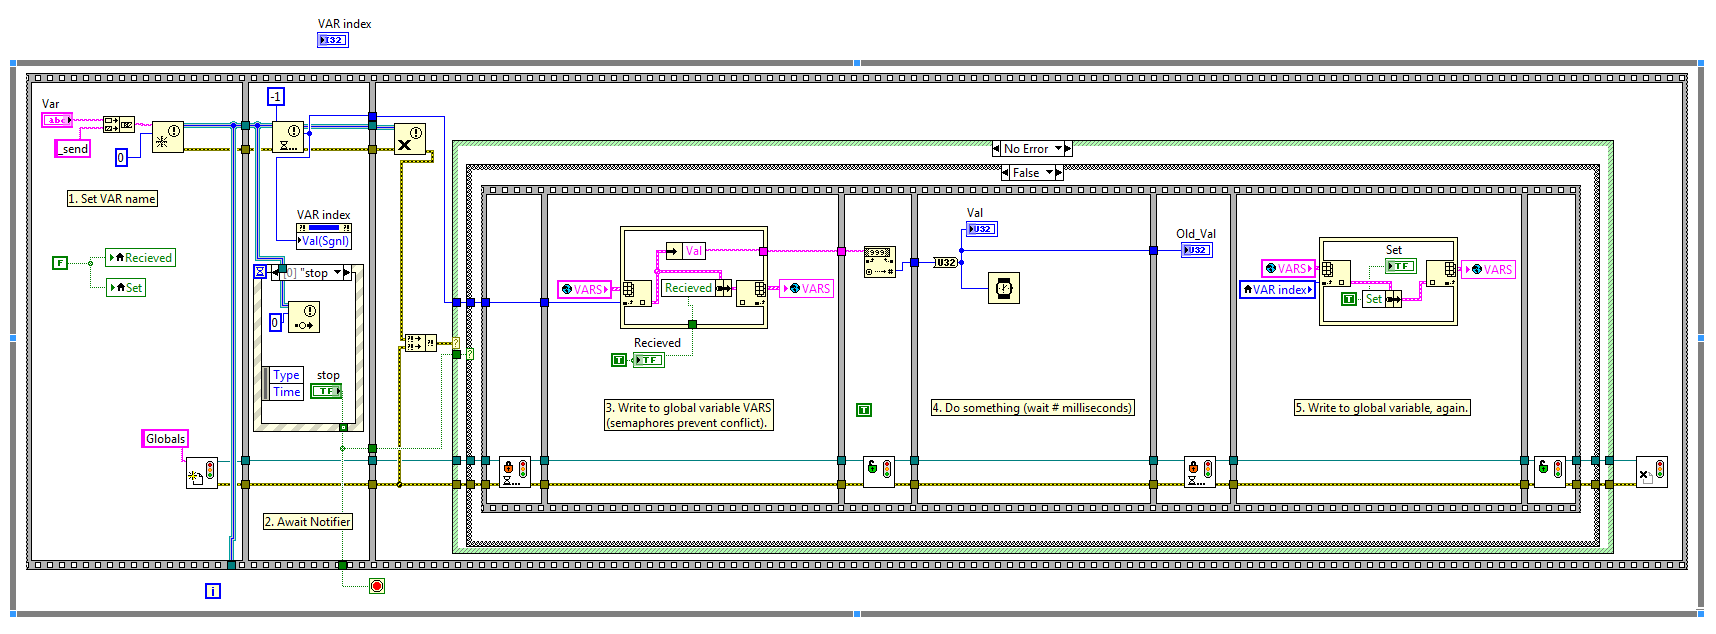
\includegraphics[width=0.9\textwidth]{images/var_block.png}

%\subsubsection{Network VARs}
%Sometimes it is not possible - or advisable - to centralise control over all experimental hardware to a single PC.  Nonetheless, hardware connected to a separate machine can still be controlled by the sequencer using Data-sockets.
\section{Writing Sequences}

\subsection[Editor.vi ]{Editor.vi \\ %
	\normalsize - simple sequence writing}
The editor provides an easy way to read/ write xml files containing sequences (.osq).  Each sequence contains an array, every element of which is a cluster that, in the simplest case, contains a comment field and the VAR\_array, e.g.

\hangindent=0.7cm
\rowcolors{1}{light-gray}{lighter-gray}
\emph{VAR array:} \\
\begin{tabularx}{0.4\textwidth}{X|X}
	\emph{Name} & \emph{Value} \\
	\hline
	VAR1 & 2 \\
	VAR2 & 3 \\
	VAR3\_OPT1 & 5 \\
	VAR3\_OPT2 & 7
\end{tabularx}
\vspace{3mm} \\
\emph{Comment:} \\
\begin{tabularx}{0.85\textwidth}{l}
	``a useful comment"
\end{tabularx}
\vspace{3mm}

To execute the above sequence line would require 3 VAR vi's to be running and listening for VAR1, VAR2, and VAR3.  The VAR3 vi would have to be able to interpret the options OPT1 and OPT2.  Every element of the seq must be written by hand, therefore Editor.vi is only really useful for writing very simple seqs, or for editing/ viewing existing .osq files.

\subsection[Modder.vi]{\label{sex:modder}Modder.vi \\ %
	\normalsize - automatic sequence building}

Modder.vi is designed to automatically write a series of instructions for the sequencer, based on all possible permutations of $n$ different variables each with $m_n$ different values.  The program works by performing a string replace on place-holder ``TAGs" written into a template sequence, with values from each row of the permutations array.  

To write a sequence, first create a template on the \emph{Sequence} tab.  The first column should contain the actual names of any VARs which are to be distributed by the sequencer, and the second column should contain the temporary TAG(s) or constant values.  The TAG can be any string, so long as it is unique within the XML version of the template sequence.  For example, for the VAR ``FOO" and TAG ``bar", create the template SEQ:

\hangindent=0.7cm
\rowcolors{1}{light-gray}{lighter-gray}
\emph{VAR array:} \\
\begin{tabularx}{0.3\textwidth}{X|X}
	\emph{Name} & \emph{Value} \\
	\hline
	FOO & bar \\
\end{tabularx}
\vspace{3mm}

Now navigate to the \emph{Permutations} tab.  Fill in a line of the \emph{Build Arrays} list, setting the field \emph{TAG} to: bar.  All values you wish to replace bar in the template can be manually entered into the \emph{Values} array, or alternatively you can populate this array automatically using the function \emph{f(x)}.  For example, set \emph{f(x)} to x+1; \emph{Steps ($m$)} to 3; change the \emph{Format} string to integer (\%d), then press \emph{Build Array}.  Notice that the \emph{Permutations} table now contains 1, 2 and 3 in the first column.  Even if you automatically populate the \emph{Values} array, you can manually add/ remove/ randomize elements afterwards. Press \emph{Make}.  This will fill the \emph{Output Seqs} array on the \emph{Sequence} tab, with each element having the template TAG replaced by a value from the permutations array.

The power of modder.vi is evident when using more than one TAG.  To see this, create another TAG and watch how the permutations table populates.  The \emph{Reorder} buttons lets you randomly order the individual arrays used to make the permutations, or alternatively the final permutation array.  This can be useful to scramble any effect of drift with your experiment, which might be misleading if the variables follow a linear series.  Keep track of how many permutations exist using the \emph{sizes} indicator; be aware this will increase very quickly as new TAGs are created!

It is not necessary to have a TAG for every VAR as you can write other VARs into the template sequence with their values set to constants.  Also, TAGS can be shared between any number of VARs, and can appear as a function if encased between `\$math' and `\$'. e.g.

\hangindent=0.7cm
\rowcolors{1}{light-gray}{lighter-gray}
\emph{VAR array:} \\
\begin{tabularx}{0.5\textwidth}{X|X}
	\emph{Name} & \emph{Value} \\
	\hline	
	ALPHA & bar \\
	BETA & \$math bar * 2 \$
\end{tabularx}
\vspace{2mm}

\noindent For the example above, \emph{Make} will replace the value for BETA with double that assigned to ALPHA.  This can be used to automatically change two variables in a correlated way.

Once a satisfactory output SEQ has been made, it can be saved to an ``.osq" file that can be read by the sequencer.  Pressing \emph{Save} will also produce an ``.omv'' file which contains the permutations array and TAG names.  This can be used in future to make similar scans with different template sequences, and is loaded using the \emph{Template *.omv file} control.  Inspect\_omv.vi and Inspect\_osq.vi allows you to plot the values saved to an omv/ osq files. This shows the parameter space that your sequence will cover.

\begin{warning} {}
	Avoid very short TAGs  (e.g. `x') as these are unlikely to be unique within the template XML.
	
	A simple system that prepends the name of the VAR it will be used with can be helpful, e.g.

	\hangindent=0.7cm
	\rowcolors{1}{light-gray}{lighter-gray}
	\emph{VAR array:} \\
	\begin{tabularx}{0.5\textwidth}{X|X}
		\emph{Name} & \emph{Value} \\
		\hline
		HV & XHV \\
	\end{tabularx}
	\vspace{2mm}
	
	This will also make it easier to guess what the TAG was used for when inspecting omv files.
\end{warning}

\subsection[Inject.vi, Append.vi, and Combine.vi]{Inject.vi, Append.vi, and Combine.vi\\ %
	\normalsize - adding lines to sequences}
Modder.vi offers a very powerful way to build sequences but it is only capable of producing rectangular permutations of the TAGs given it.  Sometimes it is convenient to make an occasional measurement with a certain set of values, e.g., to periodically measure a background during a scan.  This cannot be done with Modder.vi directly, however, Inject.vi can be used instead to add lines to .osq files at specified positions.

Load a sequence by pressing the file button on the `Open' path control.  This will populate the `SEQs' array.  Next, write the line you want to inject into this array in the `Injection' field, and fill in the `Positions' array with those where you wish the lines to go.  Now press `Inject'; scroll through `SEQs'  to check it worked.  Save as a new .osq file (or overwrite the original).

To concatenate one sequence onto the back of another use `Append.vi', which is operated in a  similar manner to `Inject.vi'.  Use `Open' to load files into the left-hand SEQ. Pressing `Append' copies the lines in the left-side SEQs to the right, or appends them to those already there.  Repeat as many times as needed to build your sequence. `Save' outputs the right-hand SEQ to file. For more advanced options with merging multiple sequences use Combine.vi. This vi takes a list of sequence files and joins together the lines from each, with the option of repeating the individual files $n$ times within the output sequence.  With `shuffle' enabled all of the lines are randomised before the output is saved.

\subsection[Filter.vi]{Filter.vi\\ %
	\normalsize - removing lines from sequences}
Filter.vi provides another way to adjust the permutations generated by modder.vi, by dropping lines according to simple logic functions.  

For instance, if you want to vary the bias applied to two electrodes (E1, E2) you can simply use Modder to create an osq file with two TAGs varied over the desired ranges.  This will generate a 2d array of EVERY possible combination of voltages, however, some of the permutations may not be useful, e.g. if E1 one must always be higher than E2 for electrons to reach a detector.  In this case, load the full .osq built by Modder.vi into Filter.vi and apply a filter that retains only the useful permutations, e.g., E1 $>$ E2, then save the output as a new sequence file.

\section{Data Acquisition}
\subsection{Integrating Data Acquisition with the Sequencer}
The process of marrying experimental control with data acquisition is very simple.  There are two methods: i) add an attribute to the HDF5 group for a given squid, which can be used to note simple single-value measurements, e.g., laser power/ lab temperature; and ii) recording of datasets, e.g., oscilloscope waveforms and camera images.  In both cases semaphores are used to prevent read/ write conflicts of the single HDF5 data file that each run produces.

\subsubsection{SQUID Attributes}
Often measurements from pressure gauges or power supplies are useful for verifying if interesting ``signals'' are real, or just arise from drifting experimental conditions.  However, lots of precise repeat measurements of the conditions might be overkill and wasteful, and a record of a single value, or the mean value, for each squid is often sufficient for monitoring.  If this is the case, such a measurement can be recorded into the attributes (meta-data) for a squid group using the global variable `Rec'.

`Rec' is a global variant that is wiped at the start of every squid.  At the end of a squid any values written to the variant during the acquisition period (using `Set variant attribute') will be appended to the attributes with the prefix \emph{REC:}.  See the example rec\_random.vi, which continuously generates a random number every 5 seconds.  Attributes with the same name are overwritten, thus the last value to be written during a given squid will be the one that is ultimately stored. Arbitrarily  many measurements can be added to the squid attributes in this way, so long as each has an unique name.

\subsubsection{Datasets}
Most scientific data will take some form of regularly sized array, such as oscilloscope waveforms, camera images, etc.  Each squid might contain many repeat measurements from the same device. In general, to record such data a VI is needed to continuously acquire data, then by reading the following global variables (written to by sequencer.vi):
\begin{description}
	\item[Save] \hfill \\
	Boolean. Is save selected in Sequencer.vi?
	\item[Acquire] \hfill \\
	Boolean. Is the Sequencer.vi state currently `acquiring data' (not, e.g., setting VARs)?
	\item[H5] \hfill \\	
	An array of paths to hdf5 file(s).   Multiple entries if sequencer.vi has several lines to \emph{Settings/Save Base} (for backing data up).
	\item[SQUID] \hfill \\
	Integer (as a string). The iterating number that uniquely identifies the current line of the running sequence.

\end{description}
it's relatively easy to coordinate the saving of data in accordance with the state of the sequencer.

For instance, you likely only wish to record data during the acquisition periods of a running SEQ, therefore in your data-acquisition VI place an appropriately configured ``h5\_[name].vi" subVI inside a case structure controlled by Save AND Running.  See `h5\_scope.vi' for example.  This VI packages the relevant meta-data (channel gain, time-base, etc.) into variant attributes and passes both this and the actual data to `H5\_1D\_SGL.vi', which then writes the data to the H5 files in a dataset called OSC\_\# (\# is replaced by the channel number), inside of the SQUID subgroup.  Something equivalent to ``h5\_scope.vi" could be made for each data-acquisition device, written to appropriately package the meta-data attributes.  LabVIEW semaphores are used to prevent more than one vi writing to the hdf5 file at the same time.  The fake\_scope.vi illustrates how this is all achieved.  fake\_camera.vi is an even simpler example that just uses the generic h5\_2D\_stacking.vi to save directly.

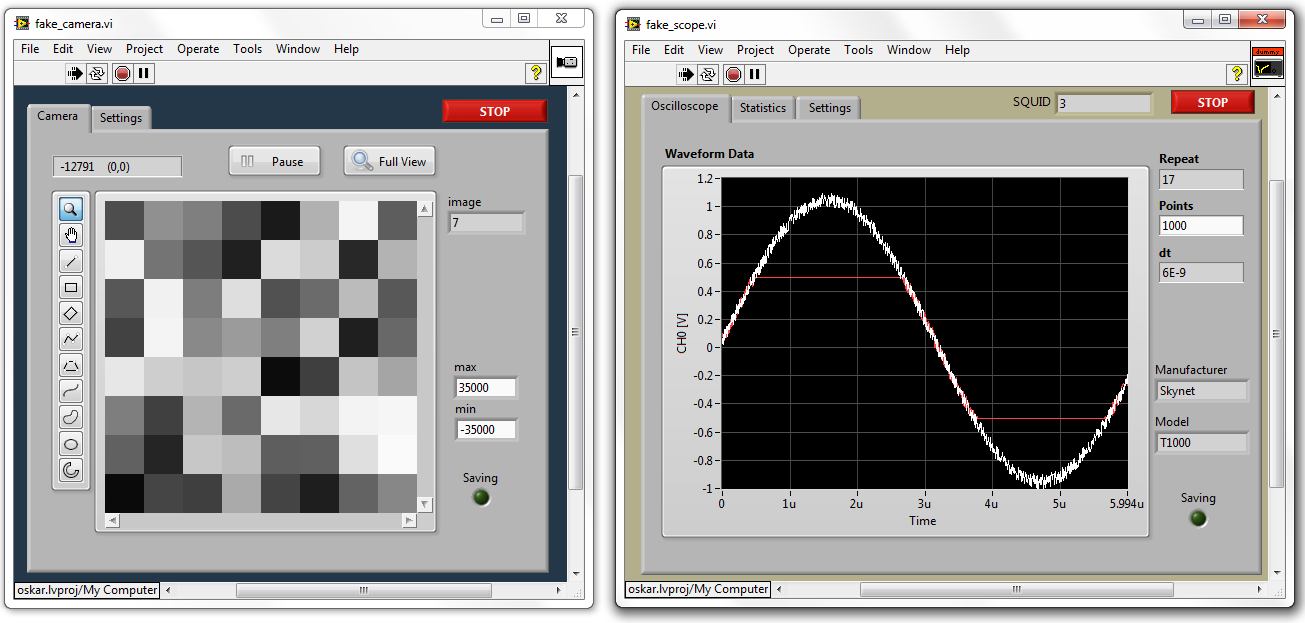
\includegraphics[width=0.9\textwidth]{images/DAQ.png}

The format for saving data depends on its shape (e.g. 1D array, 2D image) and data type (SGL, DBL, LONG, etc.).  Examples for 1D\_SGl, 1D\_DBL, 2D\_I32, can be found in the ./tools/hdf5 virtual folder.  These vi's expect repeat measurements to be made within a squid, for instance, when the 1D\_SGL is asked to write data to a pre-existing dataset, it will be appended as a new row.  The example ``h5\_stats.vi'' demonstrates how cluster data can be written to a dataset.  This might be used when, rather than a time series, a range of values (possibly of differing dtypes) are recorded at once.  This DataFrame-like structure is most likely useful if analysis is performed in LabVIEW to determine, e.g. trigger events (time, amplitude, width), or statistical features (mean, max, min, range, FWHM).

Because VAR conditions are stored in each squid's attributes, and as data relating to a squid is stored within its subgroup, it's trivial to map data to the relevant VAR conditions.  This assumes of course that data is recorded correctly, however, the individual data acquisition vi's are responsible for ensuring this (not the sequencer) and it's technically possible to get wrong.

\begin{warning}{}
	oskar is designed for experiments where many ($>$10) repeat measurements are recorded at a rate of 10 Hz to 0.3 Hz, then an experimental parameter is varied and more measurements are similarly made.  For lower acquisition rates (e.g., long camera exposure times) you must ensure that data taken near the boundary of two SQUIDS is mapped to the correct one, or safely ignored if ambiguous.  This can be done quite easily. For instance, by checking the SQUID global variable has the same value both at the start of an exposure and the end.  Alternatively, the global variable EOS (end-of-squid) can be used to synchronise the sequencer to some form of data acquisition or hardware trigger.  See `Tools/skip\_squid.vi'.  By using EOS with the acquisition time set to be unattainably long, a data acquisition device can effectively control how long the sequencer acquires data for (e.g., until 10 waveforms have been recorded).
\end{warning}


\subsection{Reviewing Data}

If everything is configured correctly a given run will produce a file called [RID]\_raw.h5, which is saved to  the folder(s) `[Base(s)]/[YYYY]/[MM]/[DD]/[RID]/'.  Opening this file using \href{https://www.hdfgroup.org/products/java/hdfview/}{HDFView} will reveal a structure akin to:

\begin{easylist}[enumerate]
	\ListProperties(Hide=100,  Hang=true, Progressive=3ex, Style*=-- ,	Style2*=$\circ$--, Style3*=$\drsh$)
	& RID~:
	&& 1
	&&& IMG
	&&& OSC\_0
	&&& OSC\_1
	&& 2
	&&& IMG
	
    \hspace{1ex} \vdots
\end{easylist}

The top level group is the RUN and has attributes, RID, SEQ FILE, AUTHOR, and DESCRIPTION.  Each group within the RUN represents a SQUID value. This has attributes DATETIME, START, END, ACQUIRE, and all appropriate VAR settings in the form, VAR:NAME = VALUE.  REC data is similarly recorded. Each SQUID group contains all of the datasets that are associated with it (OSC\_0, OSC\_1 and IMG in the example above), which could represent repeat measurements of 1D/ 2D data from oscilloscope channels or a camera.  Datasets can have their own attributes, which can be used to record, e.g., exposure time, amplifier gain, etc.  Note: the SQUID group names are strings. This is important if you wish to access a given group using, e.g., \href{http://www.h5py.org/}{h5py}.

The very structured format of HDF5 makes batch analysis a breeze.  The ability to attach meta-data makes it trivial to associate measurements with experimental conditions and instrument settings.  As HDF5 stores data in binary it's an efficient use of HDD space for whatever precision data you require, and it can be read quickly for analysis too.  It's even possible to compress data within an hdf5 file, although that has not been implemented here.  See  \href{http://h5labview.sourceforge.net/}{h5labview} docs for more info.

\addappheadtotoc
\appendix

\section{\label{sex:pseudo}Sequencer.vi pseudo-code}
The following is simplified pseudo-code illustrating the basic format of what happens when \emph{Run} is pressed in sequencer.vi.  The syntax is vaguely based on python.  The red numbered lines indicate frames within stacked sequences.
\begin{Verbatim}[commandchars=\\\{\}]
[{\color{blue}Event: Run Value Change}]
{\color{red}[0] pre-initialisation}
	global.Run = {\color{purple}True}
	global.Save = Save
	global.Acquire = {\color{purple}False}
{\color{red}[1] initilise run}
	{\color{DarkGreen}#Generate RID from timestamp}
	RID = time.now(YYYYmmdd_HHMMSS) 
	global.RID = RID
	{\color{DarkGreen}#Build path to data folder} 
	global.H5 = [`base{\textbackslash}YY{\textbackslash}MM{\textbackslash}dd{\textbackslash}RID' for base in Save_Base]
	{\color{DarkGreen}#Read osq file}
	seq = read_file(SEQ_File)
{\color{red}[2] run seq}
	loop = 1
	squid = 1
	{\color{purple}while} loop < Loops:
		{\color{purple}if} Shuffle:
			{\color{DarkGreen}#re-order seq lines}	
			seq = shuffle_seqs(seq)
		{\color{purple}for} line {\color{purple}in} seq:
			VAR_arr = line.var_array
			{\color{red}[2.0] initialise SQUID}
			global.SQUID = str(squid)
			H5[squid].write\_attributes(VAR_arr)
			{\color{DarkGreen}#create VAR string}
			var_str = var_to_str(VAR_arr)
			global.SEQLine = var_str
			{\color{purple}print}(time.now() + var_str)
			{\color{DarkGreen}#get each var name, value and options}	
			VARS = get_vars(VAR_arr)
			{\color{red}[2.1] set VARS}
			{\color{DarkGreen}#wait if pause is true}
			{\color{purple}while} Pause {\color{purple}and not} Abort:
				wait(200 ms)
			{\color{DarkGreen}#distribute VARS}
			global.VARS = VARS
			{\color{purple}for} var {\color{purple}in} VARS:
				{\color{DarkGreen}#send notifier until recieved}
				{\color{purple}while not} global.VARS[var].recieved:
					send_notifier(var.name + "\_send")
					wait(100 ms)
			{\color{DarkGreen}#wait for all vars to be set}
			{\color{purple}while not} [global.VARS.var.set for var in VARS].all():
				wait(100 ms)
			{\color{red}[2.2] acquire data}
			global.Rec = {\color{purple}None}
			global.Acquire = {\color{purple}True}
			start = time.now()
			{\color{DarkGreen}#wait for acquisition}
			{\color{purple}while} elapsed < acquire:
				end = time.now()
				elapsed = end - start
				wait(200 ms)
			global.Acquire = {\color{purple}False}
			H5[squid].write\_attributes([start, end, elapsed, global.Rec])
			{\color{red}[2.3] Reset}
			{\color{purple}for} var {\color{purple}in} VARS:
				var.set = {\color{purple}False}
				var.recieved = {\color{purple}False}
			{\color{DarkGreen}#increment squid}
			squid = squid + 1
		{\color{DarkGreen}#increment loop}
		loop = loop + 1

\end{Verbatim}

\section{\label{sex:ext}Extending the Sequencer}

It would be pretty difficult to run the experiment for which oskar's predecessor was originally designed using this version of it.  This is because that system centred around an FPGA and AO device, with dozens of outputs that would be a nightmare to individually configure using VARS.  The original solution was to have custom written controls for each SEQ line to configure these devices, encoded as voltages and DO in an array of clusters.

In principle more controls, such as the above, could be added to each SEQ line cluster, e.g.

\hangindent=0.7cm
\rowcolors{1}{light-gray}{lighter-gray}
\emph{VAR array:} \\
\begin{tabularx}{0.3\textwidth}{X|X}
	\emph{Name} & \emph{Value} \\ \hline
	RW\_A & 5 \\
	RW\_F & 9.1M \\
\end{tabularx} \\ \vspace{3mm} \\
\emph{TRAP:} \\
\begin{tabularx}{0.85\textwidth}{X|r|X|X}
	\emph{Step} & \emph{Time} & \emph{AO} & DO \\ \hline
	Accumulate & 1 & 10, 8, 7, 6.5, 50 & 0, 0, 1, 0, 0, 0 \\
	Compress & 10m & 50, 8, 7, 6.5, 50 & 0, 1, 1, 0, 0, 0 \\
	Eject & 100n & 10, 8, 7, 6.5, 50 & 0, 0, 0, 0, 0, 1 \\
\end{tabularx} \\ \vspace{3mm} \\
\emph{Comment:} \\
\begin{tabularx}{0.85\textwidth}{l}
	``a useful comment"
\end{tabularx}
\vspace{2mm}

\noindent and unbundled from it at the start of each line, then processed to appropriately configure the devices.  The quickest way to add an element is using the type-definition Tools/SEQ/Line.ctl; when you `Save' and `Apply Changes' these will propagate to the sequence editing vi's (editor, modder, etc).

Adding more elements would require adaptation of the sequencer and read/ write osq VIs.  In principle, as long as a string version of the control can be read, modder.vi will be able to write TAG values into the control (e.g. to edit a specific AO/ time-step).  Although not an insignificant amount of work, this would not be too difficult for someone with some reasonable skill with LabVIEW.

\begin{warning}{}
	Unlike creating new VARS, changing the structure of the osq cluster inevitably breaks many of the VIs which read/ write and manipulate these (XML) files.  Fortunately, this is not too difficult to fix, if you know what you're doing.
\end{warning}

In the interest of minimising dependencies, several useful features have not been  implemented in this version of oskar (they would not be too hard to add yourself).  These include support for transmitting run information to a MySQL database (LabVIEW Database Connectivity Toolkit and ODBC connector), network VARs (using Datasockets), automatic execution of analysis/ averaging scripts (System Exec.vi).
\end{document}